% このディレクトリで2回実行：pdflatex -interaction=nonstopmode -halt-on-error resume5An26w.tex
\documentclass[a4paper,10pt,pdflatex,ja=standard,jafont=ipaex-type1,
  magstyle=real,scale=1]{bxjsarticle}
\usepackage{lmodern}
\usepackage{amsmath,amssymb,mathtools}
\usepackage{geometry}
\geometry{reset,left=22mm,right=22mm,top=20mm,bottom=17mm,
  headheight=13pt,headsep=6mm,footskip=10mm}
\usepackage{xcolor}
\usepackage{enumitem}
\usepackage{array,booktabs,tabularx}
\usepackage{fancyhdr}
\usepackage{lastpage}
\usepackage{tikz}
\usetikzlibrary{arrows.meta,calc,decorations.pathreplacing}

\definecolor{ink}{HTML}{193A5C}
\definecolor{accent}{HTML}{237D82}
\definecolor{soft}{HTML}{EAF3F3}
\definecolor{muted}{HTML}{52616B}
\newcommand{\coursename}{解析学 II}
\newcommand{\handoutnumber}{5}
\pagestyle{fancy}
\fancyhf{}
\fancyhead[L]{\small\color{ink}\coursename{}・授業要約と演習}
\fancyhead[R]{\small\color{ink}第\handoutnumber 回}
\fancyfoot[C]{\small\color{ink}\thepage/\pageref{LastPage}}
\renewcommand{\headrulewidth}{0.3pt}
\setlength{\parindent}{0pt}
\setlength{\parskip}{2pt}
\setlength{\abovedisplayskip}{5pt}
\setlength{\belowdisplayskip}{5pt}
\setlength{\abovedisplayshortskip}{3pt}
\setlength{\belowdisplayshortskip}{4pt}
\setlist[itemize]{leftmargin=1.8em,itemsep=1pt,topsep=2pt,parsep=0pt}

\newcommand{\handouttitle}[1]{%
  \begin{center}
    {\Large\color{ink}#1}\par\vspace{3mm}
    {\color{accent}\rule{0.88\linewidth}{0.7pt}}
  \end{center}\vspace{-2mm}}
\newcommand{\handout}[2]{%
  \renewcommand{\handoutnumber}{#1}%
  \handouttitle{第#1回\quad #2}}
\newcommand{\topic}[1]{\par\vspace{5pt}%
  {\large\sffamily\mdseries\color{accent}#1}\par\vspace{2pt}}
\newcommand{\keybox}[1]{\par\vspace{3pt}\begingroup
  \setlength{\fboxsep}{4pt}%
  \colorbox{soft}{\parbox{\dimexpr\linewidth-2\fboxsep\relax}{\small #1}}%
  \endgroup\par\vspace{2pt}}
\newenvironment{problems}
  {\begin{enumerate}[leftmargin=2em,itemsep=3pt,topsep=3pt,parsep=0pt,
    font=\color{accent}]}
  {\end{enumerate}}


\newcommand{\examplelabel}[1]{{\sffamily\mdseries\color{ink}#1}}
\newcommand{\problemspace}{\par\vspace{5mm}}
\newcommand{\exercises}{%
  {\color{accent}\hrule height 0.7pt}\vspace{3pt}%
  \topic{演習問題（6題）}%
  {\small 特異点・無限遠を確認し、比較に使った不等式や極限を書こう。問2・3は積分値を求めなくてよい。}\par}
\tikzset{
  handout diagram/.style={>={Stealth[length=3.2pt,width=3.2pt]},line join=round,
    every node/.style={font=\scriptsize,text=ink}},
  region/.style={fill=soft,draw=accent,semithick},
  slice/.style={accent,line width=1.8pt},
  guide/.style={muted,densely dashed,thin},
  axis/.style={->,ink,thin}}


\begin{document}
\fontsize{10pt}{13.5pt}\selectfont
\setlength{\abovedisplayskip}{4pt}
\setlength{\belowdisplayskip}{4pt}
\handout{5}{広義積分}\label{lesson-start}
\keybox{到達目標：特異点と無限遠を別々の極限で扱い、収束・発散を判断できる。
関数の高さだけでなく、積分される面積の極限を調べよう。}

\topic{特異点や無限遠を極限で扱う}
有限端点では $[a,b)$、無限遠では $[a,\infty)$ の各閉部分区間で可積分な実数値関数 $f$ を考える。対応する広義積分を
$$
 \int_a^bf(x)\,dx:=\lim_{t\to b-}\int_a^tf(x)\,dx,
 \qquad
 \int_a^\infty f(x)\,dx:=\lim_{R\to\infty}\int_a^Rf(x)\,dx.
$$
と定める。有限の極限が存在するとき「収束する」という。内部の特異点 $c\in(a,b)$ は左右に分け、
両方の広義積分がそれぞれ収束する場合だけ和を取る。
$$
 \int_a^bf=\lim_{t\to c-}\int_a^tf+\lim_{s\to c+}\int_s^bf.
$$
同じ幅を除いて左右を相殺する極限は、通常の広義積分と区別する。


\par\vspace{2pt}\noindent
\begin{minipage}[b]{0.48\linewidth}\centering
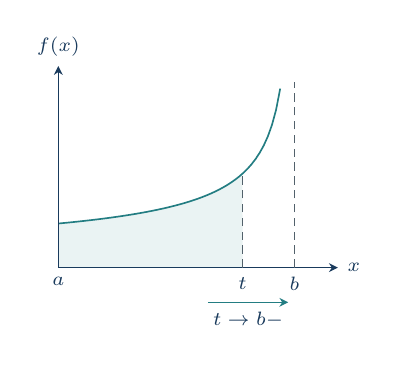
\begin{tikzpicture}[handout diagram,x=1cm,y=0.8cm]
\fill[soft] (0,0) -- plot[domain=0:0.78,samples=40] (3*\x,{0.7/sqrt(1-\x)}) -- (2.34,0) -- cycle;
 \draw[accent,semithick] plot[domain=0:0.94,samples=55] (3*\x,{0.7/sqrt(1-\x)});
 \draw[axis] (0,0) -- (3.55,0) node[right] {$x$};
 \draw[axis] (0,0) -- (0,3.2) node[above] {$f(x)$};
 \draw[guide] (2.34,0) -- (2.34,1.5);
 \draw[guide] (3,0) -- (3,2.95);
 \node[below] at (0,0) {$a$};
 \node[below] at (2.34,0) {$t$};
 \node[below] at (3,0) {$b$};
 \draw[->,accent] (1.9,-0.55) -- (2.92,-0.55) node[midway,below] {$t\to b-$};
\end{tikzpicture}\par
{\small\color{muted}端点の手前で止めてから、極限を取る}\par
\end{minipage}\hfill
\begin{minipage}[b]{0.48\linewidth}\centering
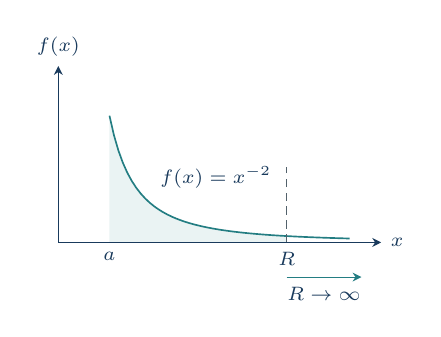
\begin{tikzpicture}[handout diagram,x=1cm,y=0.8cm]
\fill[soft] (0.65,0) -- plot[domain=0.65:2.9,samples=50] (\x,{0.85/(\x*\x)}) -- (2.9,0) -- cycle;
 \draw[accent,semithick] plot[domain=0.65:3.7,samples=55] (\x,{0.85/(\x*\x)});
 \draw[axis] (0,0) -- (4.1,0) node[right] {$x$};
 \draw[axis] (0,0) -- (0,2.8) node[above] {$f(x)$};
 \draw[guide] (2.9,0) -- (2.9,1.2);
 \node[below] at (0.65,0) {$a$};
 \node[below] at (2.9,0) {$R$};
 \node[above] at (2,0.7) {$f(x)=x^{-2}$};
 \draw[->,accent] (2.9,-0.55) -- (3.85,-0.55) node[midway,below] {$R\to\infty$};
\end{tikzpicture}\par
{\small\color{muted}上端を有限にしてから、無限遠へ広げる}\par
\end{minipage}
\par\vspace{2pt}

\topic{べき関数の収束判定と比較}
$p\in\mathbb R$ に対して、特異点付近と無限遠では条件が逆になる。
$$
 \int_0^1x^{-p}\,dx=
 \begin{cases}\dfrac1{1-p},&p<1,\\+\infty,&p\ge1,\end{cases}
 \qquad
 \int_1^\infty x^{-p}\,dx=
 \begin{cases}\dfrac1{p-1},&p>1,\\+\infty,&p\le1.\end{cases}
$$
$0\le f\le g$ なら、$\int g<\infty$ は $\int f<\infty$ を導き、
$\int f=+\infty$ は $\int g=+\infty$ を導く。
符号が変わる関数では、まず $\int|f|<\infty$（絶対収束）を調べる。


\par\vspace{2pt}\noindent
\begin{minipage}[b]{0.98\linewidth}\centering
\begin{tikzpicture}[handout diagram,x=0.75cm,y=0.62cm]
\draw[axis] (0,1.5) -- (7,1.5) node[right] {$p$};
 \draw[axis] (0,0) -- (7,0) node[right] {$p$};
 \draw[ink] (3.5,1.35) -- (3.5,1.65);
 \draw[ink] (3.5,-0.15) -- (3.5,0.15);
 \draw[slice,<-] (0.4,1.5) -- (3.35,1.5);
 \draw[slice,->] (3.65,0) -- (6.6,0);
 \node[above] at (3.5,1.5) {$1$};
 \node[above] at (3.5,0) {$1$};
 \node[left] at (0,1.5) {$\int_0^1 x^{-p}\,dx$};
 \node[left] at (0,0) {$\int_1^\infty x^{-p}\,dx$};
 \node[above] at (1.75,1.5) {収束：$p<1$};
 \node[above] at (5.15,0) {収束：$p>1$};
\end{tikzpicture}\par
{\small\color{muted}端点付近と無限遠では、収束する側が逆になる}\par
\end{minipage}
\par\vspace{2pt}

\topic{例：端点で発散しても積分は収束する}
$$
 \int_0^1\frac{dx}{\sqrt{1-x}}
 =\lim_{\varepsilon\downarrow0}
 \left[-2\sqrt{1-x}\right]_0^{1-\varepsilon}
 =\lim_{\varepsilon\downarrow0}(2-2\sqrt\varepsilon)=2.
$$
関数の値が無限大になることと、積分が発散することは同じではない。


\newpage
% 2ページ目の上半分に授業要約と例題を置く。
\noindent\begin{minipage}[b][\dimexpr0.5\textheight-\parskip\relax][t]{\linewidth}
\topic{非負関数の広義重積分}
特異点を除いた領域を $D$ とし、$D_1\subset D_2\subset\cdots$ を
有界で閉じた積分可能領域、$\bigcup_nD_n=D$ とする。各 $D_n$ 上で連続な $f\ge0$ について
$$
 \iint_Df\,dx\,dy:=\lim_{n\to\infty}\iint_{D_n}f\,dx\,dy\in[0,+\infty].
$$
非負の場合、この値は領域を増やす取り方によらない。
符号が変わる場合は $\iint_D|f|<\infty$ を仮定すれば、領域の取り方や累次積分の順序に依存しない。


\topic{例：2変数の特異点を避ける}
$D=(0,1]^2$、$D_\varepsilon=[\varepsilon,1]^2$ とすると
$$
 \iint_D\frac{dx\,dy}{\sqrt{xy}}
 =\lim_{\varepsilon\downarrow0}
 \left(\int_\varepsilon^1x^{-1/2}\,dx\right)^2
 =\lim_{\varepsilon\downarrow0}4(1-\sqrt\varepsilon)^2=4.
$$
\keybox{特異点を列挙し、各部分の極限を別々に調べる。多変数では、非負性または絶対可積分性を確認する。}

\par\vspace{2pt}\noindent
\begin{minipage}[b]{0.48\linewidth}\centering
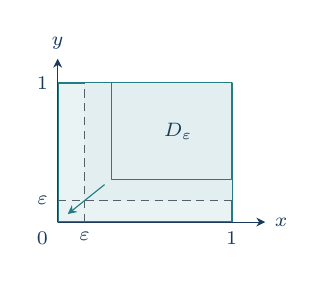
\begin{tikzpicture}[handout diagram,x=0.85cm,y=0.68cm]
\path[region] (0,0) rectangle (2.6,2.6);
 \fill[accent!13] (0.4,0.4) rectangle (2.6,2.6);
 \draw[accent] (0.8,0.8) rectangle (2.6,2.6);
 \draw[guide] (0,0.4) -- (2.6,0.4);
 \draw[guide] (0.4,0) -- (0.4,2.6);
 \draw[axis] (0,0) -- (3.1,0) node[right] {$x$};
 \draw[axis] (0,0) -- (0,3.05) node[above] {$y$};
 \node[below left] at (0,0) {$0$};
 \node[below] at (2.6,0) {$1$};
 \node[left] at (0,2.6) {$1$};
 \node[below] at (0.4,0) {$\varepsilon$};
 \node[left] at (0,0.4) {$\varepsilon$};
 \node at (1.8,1.7) {$D_\varepsilon$};
 \draw[->,accent] (0.7,0.7) -- (0.15,0.15);
\end{tikzpicture}\par
{\small\color{muted}$[\varepsilon,1]^2$ を広げ、両軸へ近づける}\par
\end{minipage}\hfill
\begin{minipage}[b]{0.48\linewidth}\centering
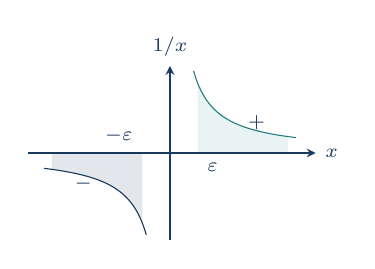
\begin{tikzpicture}[handout diagram,x=1cm,y=0.48cm]
\fill[soft] (0.35,0) -- plot[domain=0.35:1.5,samples=40] (\x,{0.65/\x}) -- (1.5,0) -- cycle;
 \fill[ink!12] (-1.5,0) -- plot[domain=-1.5:-0.35,samples=40] (\x,{0.65/\x}) -- (-0.35,0) -- cycle;
 \draw[accent] plot[domain=0.3:1.6,samples=40] (\x,{0.65/\x});
 \draw[ink] plot[domain=-1.6:-0.3,samples=40] (\x,{0.65/\x});
 \draw[axis] (-1.8,0) -- (1.85,0) node[right] {$x$};
 \draw[axis] (0,-2.3) -- (0,2.3) node[above] {$1/x$};
 \node[below right] at (0.35,0) {$\varepsilon$};
 \node[above left] at (-0.35,0) {$-\varepsilon$};
 \node at (1.1,0.8) {$+$};
 \node at (-1.1,-0.8) {$-$};
\end{tikzpicture}\par
{\small\color{muted}左右の相殺は、別々の収束を保証しない}\par
\end{minipage}
\par\vspace{2pt}

\end{minipage}\par\nointerlineskip
% 2ページ目の下半分に演習問題と書き込み用の余白を置く。
\noindent\begin{minipage}[b][0.5\textheight][t]{\linewidth}
\exercises
\begin{problems}
\item \examplelabel{極限から計算する。}
$\displaystyle\int_0^1\frac{dx}{\sqrt{x}}$、$\displaystyle\int_1^\infty\frac{dx}{x^{3/2}}$ を、
それぞれ下端を $\varepsilon>0$、上端を $R>1$ にして計算し、極限と値を求めよ。
\problemspace

\item \examplelabel{べき関数と比較する。}
(a) $\displaystyle\int_0^1\frac{dx}{\sqrt{x}(1+x)}$、
(b) $\displaystyle\int_1^\infty\frac{dx}{\sqrt{x^2+x}}$ の収束・発散を判定せよ。
(b) では $x^2+x\le2x^2$（$x\ge1$）を使う。
\problemspace

\item \examplelabel{絶対値で比較する。}
$\displaystyle\int_1^\infty\frac{\cos x}{x^{3/2}}\,dx$ が絶対収束することを示せ。
また、積分値の絶対値が $2$ 以下であることを示せ。
\problemspace


\item \examplelabel{長方形で近づける。}
$D=(0,1]^2$ とする。$D_\varepsilon=[\varepsilon,1]^2$（$0<\varepsilon<1$）で積分してから、
$\displaystyle\iint_D\frac{y}{\sqrt{x}}\,dx\,dy$ の収束と値を調べよ。
\problemspace

\item \examplelabel{無限領域へ広げる。}
$Q=[1,\infty)^2$ を $Q_R=[1,R]^2$（$R>1$）で近づけ、
(a) $\displaystyle\iint_Q\frac{dx\,dy}{x^2y^2}$、
(b) $\displaystyle\iint_Q\frac{dx\,dy}{xy}$ の収束・発散と、収束する場合の値を調べよ。
\problemspace
\item \examplelabel{特異点で分ける。}
$\displaystyle\int_{-1}^1\frac{dx}{x}$ の収束・発散を左右別々に調べよ。
$\displaystyle\int_{-1}^{-\varepsilon}\frac{dx}{x}+\int_\varepsilon^1\frac{dx}{x}=0$（$0<\varepsilon<1$）でも、収束といえないのはなぜか。（AIに聞くこと推奨）
\problemspace

\end{problems}
\end{minipage}

\newpage
\fancyhead[L]{\small\color{ink}\coursename{}・演習問題の解答}
\handouttitle{第5回\quad 演習問題の解答}
\begin{problems}
\setlength{\itemsep}{6pt}
\item \examplelabel{極限から計算する。}
$0<\varepsilon<1<R$ とすると、
$$
 \begin{aligned}
 \int_\varepsilon^1x^{-1/2}\,dx
 &=[2\sqrt{x}]_\varepsilon^1=2(1-\sqrt\varepsilon)
 \longrightarrow2\quad(\varepsilon\downarrow0),\\
 \int_1^Rx^{-3/2}\,dx
 &=[-2x^{-1/2}]_1^R=2(1-R^{-1/2})
 \longrightarrow2\quad(R\to\infty).
 \end{aligned}
$$
どちらも収束し、値は $2$。関数が端点で非有界でも、区間が無限でも、積分が発散するとは限らない。

\item \examplelabel{べき関数と比較する。}
(a) $0<x\le1$ で
$$
 0\le\frac1{\sqrt{x}(1+x)}\le x^{-1/2},\qquad
 \int_0^1x^{-1/2}\,dx=2<\infty
$$
より収束する。(b) $x\ge1$ で $x^2+x\le2x^2$ だから、
$$
 \frac1{\sqrt{x^2+x}}\ge\frac1{\sqrt2\,x},\qquad
 \int_1^\infty\frac{dx}{\sqrt2\,x}=+\infty
$$
より $+\infty$ に発散する。分母が大きいほど逆数は小さいので、不等号の向きに注意しよう。

\item \examplelabel{絶対値で比較する。}
$x\ge1$ では $|\cos x|\le1$ より、
$$
 \int_1^\infty\left|\frac{\cos x}{x^{3/2}}\right|\,dx
 \le\int_1^\infty x^{-3/2}\,dx=2<\infty.
$$
したがって絶対収束し、積分値 $I=\int_1^\infty x^{-3/2}\cos x\,dx$ は有限である。さらに、
$$
 |I|\le\int_1^\infty\frac{|\cos x|}{x^{3/2}}\,dx\le2.
$$

\item \examplelabel{長方形で近づける。}
$D_\varepsilon$ 上では連続なので、累次積分を計算できる。
$$
 \begin{aligned}
 \iint_{D_\varepsilon}\frac{y}{\sqrt{x}}\,dx\,dy
 &=\left(\int_\varepsilon^1x^{-1/2}\,dx\right)
   \left(\int_\varepsilon^1y\,dy\right)\\
 &=2(1-\sqrt\varepsilon)\,\frac{1-\varepsilon^2}{2}
 \longrightarrow1\quad(\varepsilon\downarrow0).
 \end{aligned}
$$
被積分関数は非負であり、$D_\varepsilon$ は $D$ へ広がるので、広義重積分は収束し、値は $1$。

\item \examplelabel{無限領域へ広げる。}
どちらも非負なので、$Q_R=[1,R]^2$ 上の積分の極限を調べればよい。
$$
 \begin{aligned}
 \text{(a)}\quad\iint_{Q_R}\frac{dx\,dy}{x^2y^2}
 &=\left(\int_1^Rt^{-2}\,dt\right)^2=(1-R^{-1})^2
 \longrightarrow1\quad(R\to\infty),\\
 \text{(b)}\quad\iint_{Q_R}\frac{dx\,dy}{xy}
 &=\left(\int_1^R\frac{dt}{t}\right)^2=(\log R)^2
 \longrightarrow+\infty\quad(R\to\infty).
 \end{aligned}
$$
(a) は収束し、値は $1$。(b) は $+\infty$ に発散する。同じ無限領域でも、関数の減衰の速さで結論が変わる。

\item \examplelabel{特異点で分ける。}
左右の積分を独立に調べると、
$$
 \begin{aligned}
 \int_{-1}^{-\varepsilon}\frac{dx}{x}
 &=[\log|x|]_{-1}^{-\varepsilon}=\log\varepsilon
 \longrightarrow-\infty\quad(\varepsilon\downarrow0),\\
 \int_\delta^1\frac{dx}{x}
 &=[\log x]_\delta^1=-\log\delta
 \longrightarrow+\infty\quad(\delta\downarrow0).
 \end{aligned}
$$
左右とも有限の極限をもたないので、通常の広義積分は発散する。
$\delta=\varepsilon$ とした和は $0$ だが、これは左右を同じ幅だけ除く特別な極限（コーシーの主値）である。
$-\infty$ と $+\infty$ を相殺して積分値を定めることはできない。
\end{problems}
\end{document}
